% ----------------------------------------------------------
% CONTRASTS WITH RELATED METRICS
% ----------------------------------------------------------
\section{Contrasts With Magnitude-Based Metrics}

Magnitude-based accuracy metrics, such as mean absolute error or squared error,
summarize the average deviation between forecasted and realized demand. While
these metrics are informative for assessing overall accuracy, they do not
distinguish between forecasts that fail frequently by small amounts and forecasts
that fail infrequently but by larger margins.

To illustrate this distinction, consider the two forecasting patterns shown in
Figure~\ref{fig:nsl_forecast_contrast}. Both forecasts exhibit similar aggregate
magnitude error, but their distributions of shortfalls differ substantially.
Forecast~A experiences shortfalls in only a small number of intervals, while
Forecast~B concentrates errors in several high-impact periods.

\begin{figure}[h!]
\centering
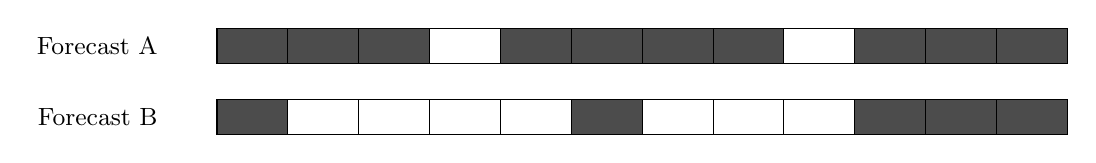
\begin{tikzpicture}[scale=0.9]

% ----------------------------------------------------------
% Forecast A (Higher NSL)
% ----------------------------------------------------------
\node[left] at (-0.7,0.25) {\small Forecast A};

% Covered intervals for Forecast A
\foreach \x in {0,1,2,4,5,6,7,9,10,11} {
    \draw[fill=black!70] (\x,0) rectangle ++(1,0.5);
}

% Shortfall intervals for Forecast A
\foreach \x in {3,8} {
    \draw[fill=white] (\x,0) rectangle ++(1,0.5);
    \draw (\x,0) rectangle ++(1,0.5);
}

% ----------------------------------------------------------
% Forecast B (Lower NSL)
% ----------------------------------------------------------
\node[left] at (-0.7,-0.75) {\small Forecast B};

% Covered intervals for Forecast B
\foreach \x in {0,5,9,10,11} {
    \draw[fill=black!70] (\x,-1) rectangle ++(1,0.5);
}

% Shortfall intervals for Forecast B
\foreach \x in {1,2,3,4,6,7,8} {
    \draw[fill=white] (\x,-1) rectangle ++(1,0.5);
    \draw (\x,-1) rectangle ++(1,0.5);
}

\end{tikzpicture}
\caption{Two forecasts with similar magnitude error but different \NSL\ values.
Forecast~A achieves coverage in 10 of 12 intervals, while Forecast~B achieves
coverage in only 5 of 12 intervals.}
\label{fig:nsl_forecast_contrast}
\end{figure}

From the perspective of \NSL, these differences are decisive. Forecast~A attains a
high \NSL\ value, indicating that demand is met reliably across most intervals.
Forecast~B yields a substantially lower \NSL, reflecting frequent shortfalls despite
comparable average error. The contrast highlights how magnitude-based metrics alone
may obscure operationally meaningful differences in forecast reliability.

This example underscores the complementary role of \NSL\ within a broader
evaluation framework. While magnitude-based metrics quantify average deviation,
\NSL\ captures the frequency with which operational requirements are satisfied.
Used together, these perspectives provide a more complete assessment of forecasting
performance than either approach alone.